
\chapter{Improved Terminal Iterative Learning Docking Control}

\section{Introduction}

\label{Introduction}

Autonomous aerial refueling (AAR) is an important method to increase the
voyage and endurance of unmanned aerial vehicles (UAVs) and avoid the conflict
between the takeoff weight and the payload weight
\cite{thomas2014advances,nalepka2005automated}. Among the aerial refueling
methods in operation today, the probe-drogue refueling (PDR)
\cite{bhandari2013bow} is the most widely adopted one owing to its flexibility
and simple requirement for equipment. There are five stages in the process of
PDR, docking is the most critical and difficult stage because it is more
susceptible to disturbances, which directly affects the success of AAR. The
docking control task is to control the probe on the receiver link up with the
drogue for fuel transfer. The docking control for PDR is a difficult task for
two main reasons. The first reason is that the system model in the docking
stage is a multi-input-multi-output (MIMO) higher-order nonlinear system with
nonminimum-phase, multi-agent, and multi-disturbance features, which is
complex for control design. Moreover, the dynamics of the receiver is slower
than that of the drogue, so it is hard for the probe on the receiver to
capture the moving drogue. The second reason is that the precision requirement
for the PDR docking control is high. The docking error should be controlled
within centimeter level, and the relative velocity between the probe and the
drogue should be controlled within a small range, such as 1$\sim$1.5 m/s
\cite{NATO-2004-3}. Therefore, the docking controller design for PDR is
important and challenging.

Many research efforts have focused on developing docking control methods for
PDR. First, the most commonly used method is the linear quadratic regulator
(LQR) \cite{tandale2006trajectory,fravolini2004modeling} because it is simple,
and the optimal feedback gain matrix can be obtained. It is a linear model
based method, and the control quality may deteriorate in the presence of large
disturbances. A second method is nonzero setpoint (NZSP)
\cite{valasek2005vision}, which transforms a tracking problem into a
stabilization problem. However, the reference state and reference input are
limited to be constant, namely the drogue is relatively static to the tanker.
It means that the receiver just needs to perform a set-point tracking task.
Some improved work is then carried out to track a moving drogue
\cite{kimmett2002vision}, but the trajectory of the drogue is assumed to be
known in advance. Thirdly, to reject complex disturbances and uncertainties
during the docking stage, active disturbance rejection control (ADRC)
\cite{su2015autonomous} and adaptive-based control
\cite{wang2007verifiable,wang2008novel} have received much attention recently.
Generally, when ADRC is applied to the trajectory tracking of aircraft, the
flight control system is designed by using scale separation. The considered
system is usually divided into several loops, which leads to a complex control
configuration. Adaptive-based control is also relatively complex. Moreover,
fault-tolerant control is also studied. A fault-tolerant adaptive model
inversion control for vision-based PDR is developed in \cite{valasek2017fault}%
. Last but not least, backstepping control is adopted in
\cite{wang2014dynamic}, which relies on the modeling precision of the PDR system.

On the whole, there still exist some challenges to designing a docking
controller for PDR. First, the PDR system is complicated. Moreover, as one of
the main disturbances in the docking stage, the bow wave effect is a
repetitive nonlinear disturbance and highly related to the states of the
receiver and the drogue, which also makes docking control difficult
\cite{dai2016modeling,wei2016drogue}. Secondly, the problem of the
\textquotedblleft slow dynamics\textquotedblright \ to track the
\textquotedblleft fast dynamics\textquotedblright \ becomes tougher if the bow
wave effect is taken into account. Some feedback control methods may result in
a chasing process between the receiver and the drogue, which may cause
overcontrol. Besides, the chasing action may lead to impact and damage to the
drogue and the probe, which is very dangerous and needs to be avoided
according to ATP-56(B) issued by NATO (North Atlantic Treaty Organisation)
\cite{NATO-2004-3}. Thirdly, there are more than twenty states in the PDR
system, so it is quite demanding for sensors to detect so many states
accurately. In practice, the global positioning system (GPS) and vision-based
navigation systems are common precise positioning methods for PDR
\cite{thomas2014advances}. Influenced by the environment, some unexpected
sensor delay may happen. Besides, real-time online state feedback is
time-consuming. As a consequence, the stability and reliability of the docking
operation may deteriorate.

In order to cope with the aforementioned three challenges, a reliable docking
control scheme for PDR is proposed in this study. Here, \textquotedblleft
reliability\textquotedblright \ means small docking error, certain robustness
against disturbances and uncertainties, little dependence on the system model
and sensors. The terminal iterative
learning control (TILC) method is utilized in the docking control scheme. TILC
has captured extensive attention from many fields since it was first presented
by \cite{Xu1999Terminal}. Iterative learning control (ILC)
\cite{Chen2012Iterative} is an effective cycle-to-cycle control approach to
achieve entire output trajectory tracking within a given time interval. When
only the end-point needs to be tracked, TILC is a good choice. In practice,
when a pilot performs a docking operation, he/she adjusts the control input or
the initial position of the receiver by learning from historical experience
and sending feedforward commands to achieve a successful docking. Similarly,
TILC gives feedforward control inputs or initial states based on the terminal output error
from the last iteration. Noteworthy, the three challenges mentioned earlier can be
solved to some extent by TILC. First, TILC is basically a model-free control
method, and little system model knowledge is required. Secondly, the control
input of the receiver is a feedforward signal, which is calculated by the
iterative learning process, so the docking safety problem caused by some
feedback control methods, which are mentioned in the last paragraph, can be
avoided. Thirdly, only terminal output information instead of all states is
needed for TILC. Besides, TILC takes advantage of the repeatability of the
docking stage. Given the advantages TILC has in tackling these challenges,
TILC is a preferable way to solve the docking control problem for PDR.

In this paper, a TILC controller is designed for the PDR system (a MIMO
higher-order nonlinear system), and convergence analysis is also carried out
without linearization. The proposed controller selects the combination of
control inputs and initial values as its learning object, which is consistent
with the pilots' operation. Besides, the iterative optimization method is
adopted to generate a suitable basis function for the proposed TILC controller
to achieve fast convergence, and to control the docking process. By combining the generation of basis function and
the proposed TILC controller, a reliable docking control scheme for PDR is established.

A previous paper of ours \cite{dai2018terminal} employed terminal iterative
learning to forecast the terminal position of the drogue and then generate the
tracking trajectory for the original autopilot system. However, it is not a
conventional TILC, and the low-level driving signals still come from the
original autopilot. There are significant differences between the work
presented in this paper and that presented in \cite{dai2018terminal}: i) The
TILC controller works as an additional unit for the trajectory generation of
the original autopilot system in \cite{dai2018terminal}, while the designed
TILC controller in this study is a low-level controller without a given
trajectory. ii) The proposed TILC controller is a hybrid controller with
control input learning and initial position learning, whereas only the docking
error learning is utilized in \cite{dai2018terminal}. iii) A basis function is
introduced into TILC for faster convergence. iv) The controlling of the x-axis
relative velocity is achieved by the trajectory planning of the x-axis
relative position rather than a saturation bound.

The main contributions of the study are twofold:

From the practical perspective, the contribution of this study is that: A
reliable docking control scheme is proposed based on TILC. With this control
scheme, the PDR system can achieve a successful docking quickly, accurately,
and safely. TILC is a kind of model-free feedforward learning control, which
can avoid the chasing action and reduce sensor burden, and thus possesses some
advantages over model-based control and real-time feedback control in terms of
the docking control problem.

From the theoretical perspective, the contribution of this study is that: TILC
design problem for a class of MIMO higher-order nonlinear system is addressed
with two key problems solved. One is that convergence analysis is carried out
without linearization; the other is that a suitable basis function is selected
by the iterative optimization method. Moreover, the partial state
controllability is also considered in the TILC design.

The paper is organized as follows. The model description and problem statement
are presented in Section \ref{ProbelmF} to transform the practical docking
control problem into a theoretical TILC control problem. Section
\ref{ControlScheme} gives a reliable docking control scheme including the
generation of the basis function and the TILC controller implementation. In
Section \ref{BasisFun}, a suitable basis function is generated for the TILC
controller. Section \ref{TILC} is devoted to the details of the TILC
controller design with the convergence analysis. Illustrative simulations are
provided in Section \ref{Simulation} to show the effectiveness of the proposed
scheme. Section \ref{Conclusions} concludes the paper.

\section{Model Description and Problem Statement}

\label{ProbelmF}

\subsection{PDR system model in the docking stage}

Fig.~\ref{Fig_Frames} and Fig.~\ref{Fig_3Views} show the PDR system, which
consists of a tanker aircraft with a flexible hose that trails behind and
below the tanker, a cone-shaped drogue mounted at the end of the hose, and a
receiver aircraft equipped with a rigid probe protruding from its nose. The
docking control task is to control the probe link up with the drogue for fuel
transfer. When establishing the PDR system model in the docking stage, three
commonly used coordinate frames are the ground frame ($o_{\text{g}}%
$-$x_{\text{g}}y_{\text{g}}z_{\text{g}}$), the tanker frame ($o_{\text{t}}%
$-$x_{\text{t}}y_{\text{t}}z_{\text{t}}$), and the drogue equilibrium-point
frame ($o_{\text{d}}$-$x_{\text{d}}y_{\text{d}}z_{\text{d}}$), which are shown
in Fig.~\ref{Fig_Frames}. The definition of these coordinate frames can be
found in \cite{wei2016drogue}.
\begin{figure}[pth]
	\begin{centering}
		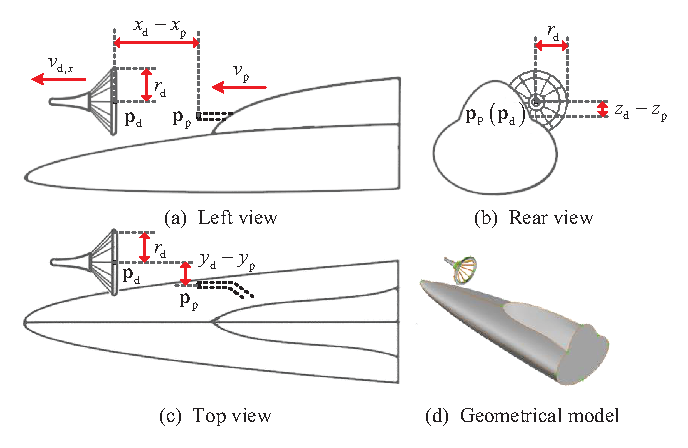
\includegraphics[width=0.6\textwidth]{Figures/Figs_Ch10/3Views} 
		\par \end{centering}
	\caption{Three views and geometrical model of the PDR system.}%
	\label{Fig_3Views}%
\end{figure}

According to \cite{stevens2004aircraft,stepanyan2004aerial}, the receiver
aircraft (F-16 aircraft is considered) is modeled as
\begin{equation}
\left \{
\begin{array}
[c]{l}%
\mathbf{\dot{x}}_{\text{r}}=\mathbf{A}_{\text{r}}\mathbf{x}_{\text{r}%
}+\mathbf{B}_{\text{r}}\mathbf{u}_{\text{r}}+\mathbf{G}_{\text{r}}%
\mathbf{f}_{\text{a}}\\
\left[
\begin{array}
[c]{c}%
\mathbf{p}_{\text{r}}\\
v_{\text{r}}%
\end{array}
\right]  =\mathbf{C}_{\text{r}}\mathbf{x}_{\text{r}}%
\end{array}
\right.  , \label{Eq_receiver}%
\end{equation}%
\begin{equation}
\left[
\begin{array}
[c]{c}%
\mathbf{p}_{\text{p}}\\
v_{\text{p}}%
\end{array}
\right]  =\left[
\begin{array}
[c]{c}%
\mathbf{p}_{\text{r}}\\
v_{\text{r}}%
\end{array}
\right]  +\left[
\begin{array}
[c]{c}%
\mathbf{p}_{\text{p/r}}\\
0
\end{array}
\right]  , \label{Eq_probe}%
\end{equation}
where $\mathbf{x}_{\text{r}}\in%
%TCIMACRO{\U{211d} }%
%BeginExpansion
\mathbb{R}
%EndExpansion
^{12}$ is the state vector of the receiver, $\mathbf{u}_{\text{r}}\in%
%TCIMACRO{\U{211d} }%
%BeginExpansion
\mathbb{R}
%EndExpansion
^{4}$ is the control input vector consisting of throttle $\delta_{\text{T}}\in%
%TCIMACRO{\U{211d} }%
%BeginExpansion
\mathbb{R}
%EndExpansion
$, elevator $\delta_{\text{e}}\in%
%TCIMACRO{\U{211d} }%
%BeginExpansion
\mathbb{R}
%EndExpansion
$, rudder $\delta_{\text{r}}\in%
%TCIMACRO{\U{211d} }%
%BeginExpansion
\mathbb{R}
%EndExpansion
$ and aileron $\delta_{\text{a}}\in%
%TCIMACRO{\U{211d} }%
%BeginExpansion
\mathbb{R}
%EndExpansion
$. The receiver mainly suffers from the atmospheric turbulence force
$\mathbf{f}_{\text{a}}\in%
%TCIMACRO{\U{211d} }%
%BeginExpansion
\mathbb{R}
%EndExpansion
^{3}$. The modeling and simulation methods for $\mathbf{f}_{\text{a}}$ have
been extensively studied in the existing literature
\cite{tandale2006trajectory,ro2010modeling}. The vector $\mathbf{p}_{\text{r}%
}=\left[  x_{\text{r}}\ y_{\text{r}}\ z_{\text{r}}\right]  ^{\text{T}}\in%
%TCIMACRO{\U{211d} }%
%BeginExpansion
\mathbb{R}
%EndExpansion
^{3}$ denotes the position of the receiver's center of mass under the tank
frame, which is combined with the velocity of the receiver $v_{\text{r}}\in%
%TCIMACRO{\U{211d} }%
%BeginExpansion
\mathbb{R}
%EndExpansion
$ to be the system output. The vector $\mathbf{p}_{\text{p}}=\left[
x_{\text{p}}\ y_{\text{p}}\ z_{\text{p}}\right]  ^{\text{T}}\in%
%TCIMACRO{\U{211d} }%
%BeginExpansion
\mathbb{R}
%EndExpansion
^{3}$ and $v_{\text{p}}\in%
%TCIMACRO{\U{211d} }%
%BeginExpansion
\mathbb{R}
%EndExpansion
$ are the position and velocity of the front-end of the probe, and
$\mathbf{p}_{\text{p/r}}\in%
%TCIMACRO{\U{211d} }%
%BeginExpansion
\mathbb{R}
%EndExpansion
^{3}$ denotes the relative position from $\mathbf{p}_{\text{r}}$ to
$\mathbf{p}_{\text{p}}$. Note that, all the system matrices $\mathbf{A}%
_{\text{r}},\mathbf{B}_{\text{r}},\mathbf{G}_{\text{r}},\mathbf{C}_{\text{r}}$
are time-invariant and of appropriate dimensions. Moreover, stability
augmentation control is often adopted for the receiver to place the poles of
the receiver system to reasonable positions in the left-half $s$-plane
\cite{stevens2004aircraft}. To this end, a state feedback matrix
$\mathbf{K}_{\text{r}}\in%
%TCIMACRO{\U{211d} }%
%BeginExpansion
\mathbb{R}
%EndExpansion
^{4\times12}$ can be designed, and then the matrix $\mathbf{A}_{\text{r}}$
becomes
\begin{equation}
\mathbf{\bar{A}}_{\text{r}}=\mathbf{A}_{\text{r}}-\mathbf{B}_{\text{r}%
}\mathbf{K}_{\text{r}}. \label{Eq_SAC}%
\end{equation}


According to \cite{wei2016drogue}, the drogue dynamics is expressed by a
transfer function, whose corresponding state-space representation is
\begin{equation}
\left \{
\begin{array}
[c]{l}%
\mathbf{\dot{x}}_{\text{d}}=\mathbf{A}_{\text{d}}\mathbf{x}_{\text{d}%
}+\mathbf{G}_{\text{d}}\left(  \mathbf{f}_{\text{b}}+\mathbf{f}_{\text{a}%
}\right) \\
\left[
\begin{array}
[c]{c}%
\mathbf{p}_{\text{d}}\\
v_{\text{d,}x}%
\end{array}
\right]  =\mathbf{C}_{\text{d}}\mathbf{x}_{\text{d}}%
\end{array}
\right.  , \label{Eq_drogue}%
\end{equation}
where $\mathbf{x}_{\text{d}}\in \mathbb{R}^{10}$ is the state of the drogue,
whose dimension is determined by the order of the fitting model in the
identification, the input $\mathbf{f}_{\text{b}}$, $\mathbf{f}_{\text{a}}\in%
%TCIMACRO{\U{211d} }%
%BeginExpansion
\mathbb{R}
%EndExpansion
^{3}$ are the bow wave effect force \cite{dogan2013bow} and the atmospheric
turbulence force. The vector $\mathbf{p}_{\text{d}}=\left[  x_{\text{d}%
}\ y_{\text{d}}\ z_{\text{d}}\right]  ^{\text{T}}\in%
%TCIMACRO{\U{211d} }%
%BeginExpansion
\mathbb{R}
%EndExpansion
^{3}$ is the position of the drogue under the tank frame, which is combined
with the velocity of the drogue in the x-axis direction of the tank frame
$v_{\text{d,}x}\in%
%TCIMACRO{\U{211d} }%
%BeginExpansion
\mathbb{R}
%EndExpansion
$ to be the system output. Similar to the receiver model, all the system
matrices $\mathbf{A}_{\text{d}},\mathbf{G}_{\text{d}},\mathbf{C}_{\text{d}}$
are time-invariant and of appropriate dimensions. Furthermore, the bow wave
effect can be represented by a nonlinear function \cite{wei2016drogue}
\begin{equation}
\mathbf{f}_{\text{b}}=\boldsymbol{\phi}_{0}\left(  \mathbf{p}_{\text{d}%
}-\mathbf{p}_{\text{p}}\right)  . \label{Eq_bowwave}%
\end{equation}
Apart from the disturbance forces $\mathbf{f}_{\text{b}}$ and $\mathbf{f}%
_{\text{a}}$, there are no other control inputs in the drogue dynamics
(\ref{Eq_drogue}). Therefore, the drogue position is passively affected by the
aerodynamic disturbances from the receiver (in a close range) and the
atmospheric environment, which is a difficulty for the docking control design.

On the whole, by combining Eqs.~(\ref{Eq_receiver}), (\ref{Eq_probe}),
(\ref{Eq_SAC}), (\ref{Eq_drogue}) and (\ref{Eq_bowwave}), a comprehensive
model for the PDR system is described as
\begin{equation}
\left \{
\begin{array}
[c]{l}%
\underset{\mathbf{\dot{x}}}{\underbrace{\left[
		\begin{array}
		[c]{c}%
		\mathbf{\dot{x}}_{\text{d}}\\
		\mathbf{\dot{x}}_{\text{r}}%
		\end{array}
		\right]  }}=\underset{\mathbf{A}}{\underbrace{\left[
		\begin{array}
		[c]{cc}%
		\mathbf{A}_{\text{d}} & \mathbf{0}\\
		\mathbf{0} & \mathbf{\bar{A}}_{\text{r}}%
		\end{array}
		\right]  }}\underset{\mathbf{x}}{\underbrace{\left[
		\begin{array}
		[c]{c}%
		\mathbf{x}_{\text{d}}\\
		\mathbf{x}_{\text{r}}%
		\end{array}
		\right]  }}+\underset{\mathbf{B}}{\underbrace{\left[
		\begin{array}
		[c]{c}%
		\mathbf{0}\\
		\mathbf{B}_{\text{r}}%
		\end{array}
		\right]  }}\underset{\mathbf{u}}{\underbrace{\mathbf{u}_{\text{r}}}}%
+\underset{\boldsymbol{\phi}\left(  \mathbf{y}\right)  }{\underbrace{\left[
		\begin{array}
		[c]{c}%
		\mathbf{G}_{\text{d}}\boldsymbol{\phi}_{0}\left(  \mathbf{p}_{\text{d}%
		}-\mathbf{p}_{\text{p}}\right) \\
		\mathbf{0}%
		\end{array}
		\right]  }}+\underset{\boldsymbol{\varphi}}{\underbrace{\left[
		\begin{array}
		[c]{c}%
		\mathbf{G}_{\text{d}}\mathbf{f}_{\text{a}}\\
		\mathbf{G}_{\text{r}}\mathbf{f}_{\text{a}}%
		\end{array}
		\right]  }}\\
\underset{\mathbf{y}}{\underbrace{\left[
		\begin{array}
		[c]{c}%
		\mathbf{p}_{\text{d}}-\mathbf{p}_{\text{p}}\\
		v_{\text{d,}x}-v_{\text{p}}%
		\end{array}
		\right]  }}=\underset{\mathbf{C}}{\underbrace{\left[
		\begin{array}
		[c]{cc}%
		\mathbf{C}_{\text{d}} & -\mathbf{C}_{\text{r}}%
		\end{array}
		\right]  }}\underset{\mathbf{x}}{\underbrace{\left[
		\begin{array}
		[c]{c}%
		\mathbf{x}_{\text{d}}\\
		\mathbf{x}_{\text{r}}%
		\end{array}
		\right]  }}+\underset{\mathbf{d}}{\underbrace{\left[
		\begin{array}
		[c]{c}%
		\mathbf{-p}_{\text{p/r}}\\
		\mathbf{0}%
		\end{array}
		\right]  }}%
\end{array}
\right.  . \label{Eq_PDRsys}%
\end{equation}
When Eq.~(\ref{Eq_PDRsys}) is established in the drogue equilibrium-point
frame, the initial states are
\begin{equation}
\mathbf{x}_{\text{d}}\left(  0\right)  =\mathbf{0,x}_{\text{r}}\left(
0\right)  =\mathbf{x}_{\text{r0}}. \label{Eq_X0}%
\end{equation}
The physical meaning of Eq.~(\ref{Eq_X0}) is that: when $t=0$, the drogue is
still and steady, and the receiver stays away from the drogue at an initial
position $\mathbf{x}_{\text{r0}}$.

In practice, it is expected that the docking process lasts from
$t_{\text{start}}$ to $t_{\text{end}}$. The docking stage terminates when%
\begin{equation}
t_{\text{dock}}=\underset{t}{\arg}\min \left \vert x_{\text{d}}\left(  t\right)
-x_{\text{p}}\left(  t\right)  \right \vert , \label{Eq_tdock}%
\end{equation}
which is expected to be equal to $t_{\text{end}}$ (desired docking moment). At
this moment, if%
\begin{equation}%
\begin{array}
[c]{l}%
e_{\text{dock}}=\left \Vert \left[  y_{\text{d}}\left(  t_{\text{dock}}\right)
\ z_{\text{d}}\left(  t_{\text{dock}}\right)  \right]  ^{\text{T}}-\left[
y_{\text{p}}\left(  t_{\text{dock}}\right)  \ z_{\text{p}}\left(
t_{\text{dock}}\right)  \right]  ^{\text{T}}\right \Vert <r_{\text{d}},\\
-v_{\text{max}}<v_{\text{d,}x}\left(  t_{\text{dock}}\right)  -v_{\text{p}%
}\left(  t_{\text{dock}}\right)  <-v_{\text{min}},
\end{array}
\label{Eq_Criteria}%
\end{equation}
the docking attempt is regarded as successful \cite{Dibley-2007-2}, where
$v_{\text{max}},v_{\text{min}}$ are the threshold of relative velocity to open
the fuel valve at the docking moment, and $r_{\text{d}}$ is the radius of the
drogue as shown in Fig.~\ref{Fig_3Views}.

\subsection{TILC problem statement}

Regarding the control design, there are four outputs $x_{\text{d/p}%
},y_{\text{d/p}},z_{\text{d/p}},v_{\text{d}x\text{/p}}$ ($\mathbf{p}%
_{\text{d}}-\mathbf{p}_{\text{p}}\triangleq \lbrack x_{\text{d/p}%
}\ y_{\text{d/p}}\ z_{\text{d/p}}]^{\text{T}},v_{\text{d,}x}-v_{\text{p}%
}\triangleq v_{\text{d}x\text{/p}}$) to be controlled. The controlling of
$v_{\text{d}x\text{/p}}$ can be achieved by the trajectory planning of
$x_{\text{d/p}}$. Thus, the following system from (\ref{Eq_PDRsys}) is left to
be considered%
\begin{equation}
\left \{
\begin{array}
[c]{l}%
\mathbf{\dot{x}}=\mathbf{Ax}+\mathbf{Bu}+\boldsymbol{\phi}\left(
\mathbf{\bar{y}}\right)  +\boldsymbol{\varphi}\\
\mathbf{\bar{y}}=\mathbf{\bar{C}x}+\mathbf{\bar{d}}%
\end{array}
\right.  , \label{Eq_PDRSys2}%
\end{equation}
where $\mathbf{\bar{y}}=\left[  x_{\text{d/p}}\ y_{\text{d/p}}\ z_{\text{d/p}%
}\right]  ^{\text{T}},\mathbf{u}=\left[  \delta_{\text{T}}\  \delta_{\text{e}%
}\  \delta_{\text{a}}\text{ }\delta_{\text{r}}\right]  ^{\text{T}}$,
$\mathbf{\bar{C}}$ is generated from $\mathbf{C}$ by removing the last row,
$\mathbf{\bar{d}}$ is generated from $\mathbf{d}$ by removing the last row.

According to Section \ref{Introduction}, TILC is a preferable way to solve the
docking control problem. Thus, system (\ref{Eq_PDRSys2}) is rewritten as a
model for controller design:
\begin{equation}
\left \{
\begin{array}
[c]{l}%
\mathbf{\dot{x}}_{k}\left(  t\right)  =\mathbf{Ax}_{k}\left(  t\right)
+\mathbf{Bu}_{k}\left(  t\right)  +\boldsymbol{\phi}\left(  \mathbf{\bar{y}%
}_{k}\left(  t\right)  \right)  +\boldsymbol{\varphi}_{k}\\
\mathbf{\bar{y}}_{k}\left(  t\right)  =\mathbf{\bar{C}x}_{k}\left(  t\right)
+\mathbf{\bar{d}},\mathbf{x}_{k}\left(  0\right)  =\mathbf{x}_{0,k}%
\end{array}
\right.  , \label{E_OriginalSystem}%
\end{equation}
where $t\in \left[  0,T\right]  $ is the time with the cycle period
$T=t_{\text{end}}-t_{\text{start}}$, the subscript $k\in%
%TCIMACRO{\U{2115} }%
%BeginExpansion
\mathbb{N}
%EndExpansion
_{+}$ is the cycle number, $\mathbf{x}_{k}\in%
%TCIMACRO{\U{211d} }%
%BeginExpansion
\mathbb{R}
%EndExpansion
^{22}$, $\mathbf{u}_{k}\in%
%TCIMACRO{\U{211d} }%
%BeginExpansion
\mathbb{R}
%EndExpansion
^{4}$, $\mathbf{\bar{y}}_{k}\in%
%TCIMACRO{\U{211d} }%
%BeginExpansion
\mathbb{R}
%EndExpansion
^{3}$. The desired terminal output $\mathbf{\bar{y}}_{\text{d}}\left(
T\right)  $ is known. Henceforth, for convenience, the variables $t$ and $k$
will be omitted except when necessary. The following assumptions are made on
system (\ref{E_OriginalSystem}).

\textbf{Assumption 1. }The initial state $\mathbf{x}_{k}\left(  0\right)  $
can be reset at every iteration $k$.

\textbf{Assumption 2. }The atmospheric turbulence force is bounded and\textbf{
}$\left \Vert \boldsymbol{\varphi}_{k}-\boldsymbol{\varphi}_{k-1}\right \Vert
\leq D$.

\textbf{Assumption 3. }The function $\boldsymbol{\phi(}\mathbf{\bar{y})}$
satisfies the local Lipschitz condition on $M$, namely $\left \Vert
\boldsymbol{\phi}\left(  \mathbf{\bar{y}}_{k}\right)  -\boldsymbol{\phi
}\left(  \mathbf{\bar{y}}_{k-1}\right)  \right \Vert \leq l_{\boldsymbol{\phi}%
}\left \Vert \mathbf{\bar{y}}_{k}-\mathbf{\bar{y}}_{k-1}\right \Vert $, where
$M=\left \{  \mathbf{\bar{y}}\left \vert \mathbf{\bar{y}-\bar{y}}_{\text{d}%
}\left(  T\right)  \in \mathcal{B}\left(  \mathbf{0}_{3\times1},\delta \right)
\right.  \right \}  $ is an open connected set with $\mathcal{B}\left(
\mathbf{0}_{3\times1},\delta \right)  \triangleq \left \{  \boldsymbol{\xi}\in%
%TCIMACRO{\U{211d} }%
%BeginExpansion
\mathbb{R}
%EndExpansion
^{3}\left \vert \left \Vert \boldsymbol{\xi}-\mathbf{0}_{3\times1}\right \Vert
\leq \delta,\delta \in%
%TCIMACRO{\U{211d} }%
%BeginExpansion
\mathbb{R}
%EndExpansion
_{+}\right.  \right \}  $ denoting a neighborhood with the radius $\delta$
around the origin $\mathbf{0}_{3\times1}$, and $l_{\boldsymbol{\phi}}$ is a
positive Lipschitz constant.

In practice, if a docking attempt fails, the receiver will retreat to the
standby position for the next attempt \cite{dai2018terminal}, which means the
initial state $\mathbf{x}_{k}\left(  0\right)  $ can be reset at every
iteration $k$, namely \textit{Assumption 1}. The
initial state $\mathbf{x}_{k}\left(  0\right)  $ can be measured by various types of sensors, for example vision-based systems \cite{valasek2017fault}. \textit{Assumption 2 }is an
assumption on the disturbance $\boldsymbol{\varphi}$. It is well known that
ILC can remove repetitive disturbances. Thus one only needs to know the
variations of disturbances in any two consecutive cycles. \textit{Assumption
	2} describes the bounds of such variations. Because the docking operation is
just allowed in calm days, atmospheric turbulence force can be bounded
\cite{tandale2006trajectory,ro2010modeling}. As for \textit{Assumption 3}, the
nonlinear term $\boldsymbol{\phi(}\mathbf{\bar{y})}$ comes from the bow wave
effect, whose concrete expression satisfies the local Lipschitz condition
\cite{wei2016drogue}. Thus, all the three assumptions above are reasonable for
the PDR docking control problem.

For an actual PDR system, the drogue position and the relative position between the probe and the drogue are usually measured by vision-based sensors whose measurement precision depends on the relative distance (higher precision in the closer distance). Therefore, compared with the trajectory data, the terminal positions of the probe and the drogue are usually easier to measure in practice. Then, the controller directly uses the terminal docking error (relative position between the drogue and the probe at the docking moment) to give the next control input. Filters can also be used to remove the sensor noise.

\textbf{Objective.} The control objective is to construct a sequence of
control $\mathbf{u}_{k}\left(  t\right)  ,$ $t\in \left[  0,T\right]  $ for
system (\ref{E_OriginalSystem}) such that
\begin{equation}
\left \Vert \mathbf{\bar{y}}_{\text{d}}\left(  T\right)  -\mathbf{\bar{y}}%
_{k}\left(  T\right)  \right \Vert <r_{\text{d}}\text{ as }k\rightarrow
\infty \text{,} \label{E_Objective}%
\end{equation}
where $\mathbf{\bar{y}}_{k}\left(  T\right)  $ is the corresponding output at
the terminal time $T$ driven by $\mathbf{u}_{k}\left(  t\right)  $.

\section{A Reliable Docking Control Scheme}

\label{ControlScheme}

With the control problem (\ref{E_Objective}) in hand, a docking control scheme
aiming for fast and reliable PDR docking is put forward in this section, which
is depicted in Fig.~\ref{Fig_ControlScheme}. The control scheme includes two parts:

(i) Design a TILC controller to achieve the control objective
(\ref{E_Objective}).

(ii) Generate a basis function for the designed TILC controller to obtain
fast convergence, and to control the docking process.

The generation of the basis function matrix belongs to the preparation stage
of docking control, and the designed TILC controller works in the
implementation stage of docking control. In\textbf{ }the\textbf{ }preparation
stage, there is no need to consider the complex PDR model directly. The
receiver system with SAC (\ref{Eq_receiverSAC}) is considered to get a
suitable basis function for the TILC design based on the actual PDR system
in the implementation stage. Through the preparation work, a
satisfactory basis function can be attained offline before the docking
operation. During the implementation stage, the designed TILC
controller works in a repetitive and learning way to achieve a successful
docking eventually. Based on the established basis function matrix, the TILC
controller is simple and easy to apply. The details of the two parts of the
proposed docking control scheme will be described in the subsequent
sections.\begin{figure}[pth]
	\begin{centering}
		\includegraphics[width=0.6\textwidth]{Figures/Figs_Ch10/ControlScheme} 
		\par \end{centering}
	\caption{A TILC-based reliable docking control scheme.}%
	\label{Fig_ControlScheme}%
\end{figure}

\section{Offline Generation of Basis Function}

\label{BasisFun}

A better basis function leads to a faster convergence for TILC. Since the
iterative process of the docking control for PDR is expected to be
successfully finished within 2$\sim$3 attempts, the basis function
$\mathbf{U}_{\text{b}}\left(  t\right)  $ should be carefully selected here.
Regarding the selection of the basis function, the common practice is: First,
the output profile is parameterized into a polynomial or other functions.
Then, the unknown parameters in the proposed function are calculated based on
known conditions, which means the output profile is determined. Finally, with
the known output profile and a simplified system model, one may obtain the
corresponding input which can be used to determine a suitable basis function
\cite{Xu1999Terminal}. In this section, a suitable basis function matrix is
chosen by iterative optimization method for better performance. First, a
reference docking trajectory $\mathbf{p}_{\text{r,r}}\left(  t\right)  $
should be provided. Then, it is aimed to obtain the corresponding reference
inputs leading to the given reference docking trajectory $\mathbf{p}%
_{\text{r,r}}\left(  t\right)  $, and the obtained reference inputs make up
the desired basis function matrix $\mathbf{U}_{\text{b}}\left(  t\right)  $.

A reference docking trajectory is a reasonable smooth flight trajectory for
the receiver to finish the docking task. To this end, the existing work
mainly adopts three methods: low-pass filter method
\cite{fravolini2003development}, polynomial interpolation method
\cite{fravolini2004modeling}, terminal guidance method \cite{ochi2005flight}.
To establish basis function matrix $\mathbf{U}_{\text{b}}\left(  t\right)  $,
a reference output trajectory $\mathbf{p}_{\text{r,r}}\left(  t\right)  $ is
pre-designed to satisfy the docking requirements of PDR systems and especially
to guarantee the terminal docking error. Such a reference output trajectory
also needs to give a docking relative velocity of 1$\sim$1.5 m/s. The
generation of reference docking trajectory is well studied and omitted here.

As mentioned in Section \ref{Introduction}, ILC is a method to generate inputs
that can achieve a perfect tracking of the reference docking trajectory.
However, the receiver is nonminimum-phase, so adjoint-type ILC is considered
here. For the receiver with SAC%
\begin{equation}
\left \{
\begin{array}
[c]{l}%
\mathbf{\dot{x}}_{\text{r}}=\mathbf{\bar{A}}_{\text{r}}\mathbf{x}_{\text{r}%
}+\mathbf{B}_{\text{r}}\mathbf{u}_{\text{r}}\\
\mathbf{p}_{\text{r}}=\mathbf{\bar{C}}_{\text{r}}\mathbf{x}_{\text{r}}%
\end{array}
\right.  , \label{Eq_receiverSAC}%
\end{equation}
an adjoint-type ILC is designed as%
\begin{equation}
\mathbf{u}_{\text{r,}k\text{+1}}=\mathbf{u}_{\text{r,}k}+\alpha_{k}%
\mathcal{G}^{\ast}\left(  \mathbf{p}_{\text{r,r}}\left(  t\right)
-\mathbf{p}_{\text{r}}\left(  t\right)  \right)  , \label{Eq_AdjointILC}%
\end{equation}
where $\mathbf{u}_{\text{r}}=\left[  \delta_{\text{T}}\  \delta_{\text{e}%
}\  \delta_{\text{a}}\  \delta_{\text{r}}\right]  ^{\text{T}}$, $\mathbf{\bar
	{C}}_{\text{r}}$ is generated from $\mathbf{C}_{\text{r}}$ by removing the
last row, $\mathcal{G}$ is the operator of system (\ref{Eq_receiverSAC}),
$\mathcal{G}^{\ast}$ is the adjoint operator of $\mathcal{G}$. One can refer
to \cite{wei2017output} for the selection of $\alpha_{k}$ and other details.
After twenty offline iterations, the actual outputs track the reference
docking trajectory completely as shown in Fig.~\ref{Fig_Output_iter}. The
corresponding reference inputs $\delta_{\text{T,r}},\delta_{\text{a,r}}%
,\delta_{\text{e,r}},\delta_{\text{r,r}}$ are depicted in
Fig.~\ref{Fig_Input_outerloop}. Then, the desired basis function matrix is
obtained as
\begin{equation}
\mathbf{U}_{\text{b}}\left(  t\right)  =\left[
\begin{array}
[c]{cccc}%
\delta_{\text{T,r}}\left(  t\right)  & 0 & 0 & 0\\
0 & \delta_{\text{a,r}}\left(  t\right)  & 0 & 0\\
0 & 0 & \delta_{\text{e,r}}\left(  t\right)  & 0\\
0 & 0 & 0 & \delta_{\text{r,r}}\left(  t\right)
\end{array}
\right]  . \label{E_Ub}%
\end{equation}
\begin{figure}[pth]
	\begin{centering}
		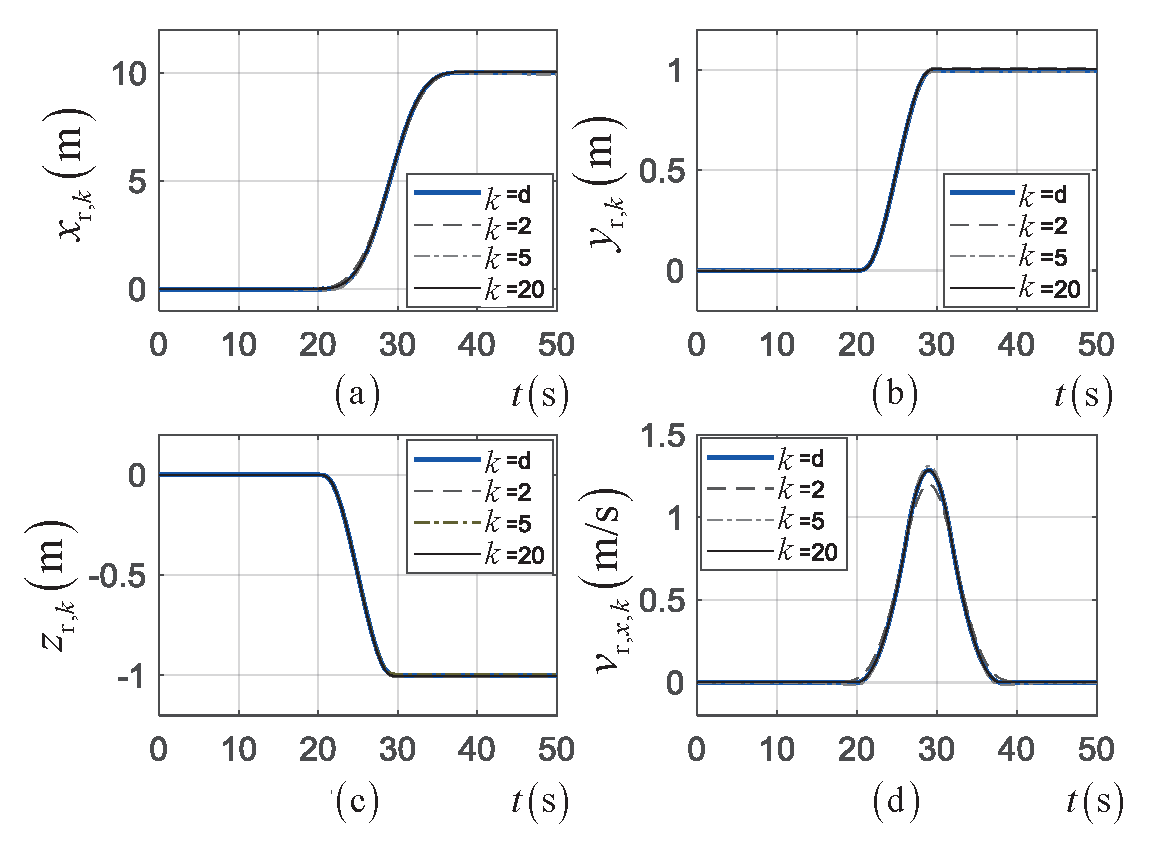
\includegraphics[width=0.6\textwidth]{Figures/Figs_Ch10/Output_iter} 
		\par \end{centering}
	\caption{Iterative tracking for the given reference docking trajectory $\mathbf{p}_{\text{r,r}}\left(  t\right)  $ by the adjoint-type ILC.}%
	\label{Fig_Output_iter}%
\end{figure}\begin{figure}[pth]
	\begin{centering}
		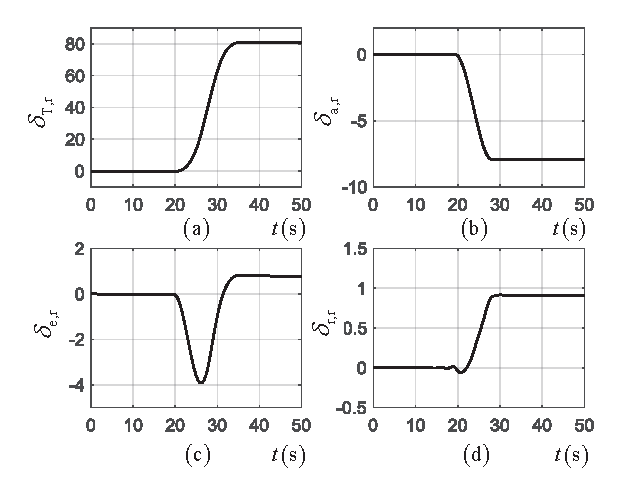
\includegraphics[width=0.6\textwidth]{Figures/Figs_Ch10/Input_outerloop} 
		\par \end{centering}
	\caption{Reference inputs leading to the given reference docking trajectory
		$\mathbf{p}_{\text{r,r}}\left(  t\right)  $.}%
	\label{Fig_Input_outerloop}%
\end{figure}

In practice, in the presence of successful docking experiences, one can
directly select a practical docking trajectory as a reference docking
trajectory $\mathbf{p}_{\text{r,r}}\left(  t\right)  $ and then obtain the
corresponding basis function $\mathbf{U}_{\text{b}}\left(  t\right)  $, or
select a practical pilots' operation as the basis function $\mathbf{U}%
_{\text{b}}\left(  t\right)  $.

Until now, the desired basis function matrix $\mathbf{U}_{\text{b}}\left(
t\right)  $ has been generated, namely the preparation work of docking control
has been done. Next, a TILC controller based on the generated basis function
matrix $\mathbf{U}_{\text{b}}\left(  t\right)  $ is to be designed.

\section{TILC Controller Design}

\label{TILC}

This section presents the TILC controller design for the MIMO higher-order
nonlinear system (\ref{E_OriginalSystem}) to achieve the control objective
(\ref{E_Objective}). For most of the time, traditional TILC controllers use
the control input or initial state value as their learning object, while a
hybrid TILC controller aiming to improve the controller performance by a
combined learning object is developed in this paper. Taking the proposed TILC
controller into consideration, the overall closed-loop block diagram of a PDR
system during the docking process is depicted in Fig.~\ref{Fig_SimStrDiagram}.
\begin{figure}[pth]
	\begin{centering}
		\includegraphics[width=0.6\textwidth]{Figures/Figs_Ch10/Simulation_structure_diagram} 
		\par \end{centering}
	\caption{Closed-loop system block diagram of a PDR system with the proposed
		TILC controller.}%
	\label{Fig_SimStrDiagram}%
\end{figure}

In general, only partial initial states are controllable, such as, in the
docking stage, the initial position of the receiver is controllable. The
initial position of the receiver can be changed in every docking attempt to
perform a successful docking. According to the state controllability, the
initial state can be rewritten as
\begin{equation}
\mathbf{x}_{0,k}=\left[  \boldsymbol{\xi}^{\text{T}}\  \boldsymbol{\eta}%
_{k}^{\text{T}}\right]  ^{\text{T}}=\mathbf{M}_{1}\boldsymbol{\xi}%
+\mathbf{M}_{2}\boldsymbol{\eta}_{k}, \label{E_Init}%
\end{equation}
where $\boldsymbol{\xi}\in%
%TCIMACRO{\U{211d} }%
%BeginExpansion
\mathbb{R}
%EndExpansion
^{19}$ denotes the uncontrollable initial state, and $\boldsymbol{\eta}_{k}\in%
%TCIMACRO{\U{211d} }%
%BeginExpansion
\mathbb{R}
%EndExpansion
^{3}$ ($\mathbf{p}_{\text{r}}$) denotes the controllable initial state, which
will be utilized in the next iteration; $\mathbf{M}_{1}=\left[  \mathbf{I}%
_{19}^{\text{T}}\  \mathbf{0}_{3\times19}^{\text{T}}\right]  ^{\text{T}},$
$\mathbf{M}_{2}=\left[  \mathbf{0}_{19\times3}^{\text{T}}\  \mathbf{I}%
_{3}^{\text{T}}\right]  ^{\text{T}}$. The system whose initial state does not
fit the order can be transformed into the form of (\ref{E_Init}) by changing
the state order.

The learning control law for system (\ref{E_OriginalSystem}) is designed as
\begin{equation}
\mathbf{u}_{k}\left(  t\right)  =\mathbf{U}_{\text{b}}\left(  t\right)
\mathbf{q}_{k}, \label{E_ControlLaw_C3}%
\end{equation}
where $\mathbf{q}_{k}\in%
%TCIMACRO{\U{211d} }%
%BeginExpansion
\mathbb{R}
%EndExpansion
^{4}$ is a constant parameter vector, $\mathbf{U}_{\text{b}}\left(  t\right)
\in%
%TCIMACRO{\U{211d} }%
%BeginExpansion
\mathbb{R}
%EndExpansion
^{4\times4}$ is a diagonal basis function matrix, which has been generated in
the last section.

Because the combination of the control input and initial state value is chosen
as the learning object, the learning update law of $\mathbf{q}_{k}$ and
$\boldsymbol{\eta}_{k}$ is proposed as
\begin{equation}
\left[
\begin{array}
[c]{c}%
\mathbf{q}_{k}\\
\boldsymbol{\eta}_{k}%
\end{array}
\right]  =\left[
\begin{array}
[c]{c}%
\mathbf{q}_{k-1}\\
\boldsymbol{\eta}_{k-1}%
\end{array}
\right]  +\left[
\begin{array}
[c]{c}%
\mathbf{L}_{1}\\
\mathbf{L}_{2}%
\end{array}
\right]  \mathbf{e}_{k-1}\left(  T\right)  \text{,} \label{E_LearningLaw_C3}%
\end{equation}
where $\mathbf{L}_{1}\in%
%TCIMACRO{\U{211d} }%
%BeginExpansion
\mathbb{R}
%EndExpansion
^{4\times3}$, $\mathbf{L}_{2}\in%
%TCIMACRO{\U{211d} }%
%BeginExpansion
\mathbb{R}
%EndExpansion
^{3\times3}$ are constant parameter matrices, $\mathbf{e}_{k}\left(  T\right)
\triangleq \mathbf{\bar{y}}_{\text{d}}\left(  T\right)  -\mathbf{\bar{y}}%
_{k}\left(  T\right)  $ is the docking error. Then, the following theorem
provides the convergence condition of the designed controller including
Eqs.~(\ref{E_ControlLaw_C3}) and (\ref{E_LearningLaw_C3}).

\textbf{Theorem 1. }For system (\ref{E_OriginalSystem}), suppose that i)
\textit{Assumptions 1-3} are satisfied; ii) the control law and update law of
TILC are designed as Eq.~(\ref{E_ControlLaw_C3}) and
Eq.~(\ref{E_LearningLaw_C3}), respectively. If the following inequality
\begin{equation}
\alpha+\gamma<1 \label{Eq_Condition3}%
\end{equation}
holds, then the docking error%
\begin{equation}
\left \Vert \mathbf{e}_{k}\left(  T\right)  \right \Vert \rightarrow
\frac{\varepsilon}{1-\alpha-\gamma} \label{E_e_docking}%
\end{equation}
as $k\rightarrow \infty,$ where
\begin{align*}
\alpha &  =\left \Vert \mathbf{I}_{3}-\mathbf{\bar{C}M}_{2}\mathbf{L}_{2}-%
%TCIMACRO{\dint \nolimits_{0}^{T}}%
%BeginExpansion
{\displaystyle \int \nolimits_{0}^{T}}
%EndExpansion
\mathbf{\bar{C}BU}_{\text{b}}\left(  \tau \right)  \mathbf{L}_{1}\text{d}%
\tau \right \Vert ,\\
\gamma &  =%
%TCIMACRO{\dint \nolimits_{0}^{T}}%
%BeginExpansion
{\displaystyle \int \nolimits_{0}^{T}}
%EndExpansion
\left(  \left \Vert \mathbf{\bar{C}A}\right \Vert +l_{\boldsymbol{\phi}%
}\left \Vert \mathbf{\bar{C}}\right \Vert ^{2}\right)  \beta \left(  \tau \right)
\text{d}\tau,\\
\beta \left(  t\right)   &  =\left \Vert \mathbf{M}_{2}\mathbf{L}_{2}\right \Vert
e^{\left(  \left \Vert \mathbf{A}\right \Vert +l_{\boldsymbol{\phi}}\left \Vert
	\mathbf{\bar{C}}\right \Vert \right)  t}+%
%TCIMACRO{\dint \nolimits_{0}^{t}}%
%BeginExpansion
{\displaystyle \int \nolimits_{0}^{t}}
%EndExpansion
e^{\left(  \left \Vert \mathbf{A}\right \Vert +l_{\boldsymbol{\phi}}\left \Vert
	\mathbf{\bar{C}}\right \Vert \right)  \left(  t-\tau \right)  }\left \Vert
\mathbf{BU}_{\text{b}}\left(  \tau \right)  \mathbf{L}_{1}\right \Vert
\text{d}\tau,\\
\varepsilon &  =DT\left \Vert \mathbf{\bar{C}}\right \Vert +%
%TCIMACRO{\dint \nolimits_{0}^{T}}%
%BeginExpansion
{\displaystyle \int \nolimits_{0}^{T}}
%EndExpansion
\left(  \left \Vert \mathbf{\bar{C}A}\right \Vert +l_{\boldsymbol{\phi}%
}\left \Vert \mathbf{\bar{C}}\right \Vert ^{2}\right)  DTe^{\left(  \left \Vert
	\mathbf{A}\right \Vert +l_{\boldsymbol{\phi}}\left \Vert \mathbf{\bar{C}%
	}\right \Vert \right)  \tau}\text{d}\tau.
\end{align*}
Moreover, if there is no atmospheric turbulence disturbance, namely $D=0$,
$\varepsilon=0$, then $\left \Vert \mathbf{e}_{k}\left(  T\right)  \right \Vert
\rightarrow0$.

\textit{Proof}. Refer to \textit{Appendix A}. $\square$

Because of the introduction of basis function matrix $\mathbf{U}_{\text{b}%
}\left(  t\right)  $, the iterative learning object is transformed from the
control input $\mathbf{u}_{k}\left(  t\right)  $ to a parameter vector
$\mathbf{q}_{k}$, which makes the controller implementation simpler. Besides,
because the basis function matrix $\mathbf{U}_{\text{b}}\left(  t\right)  $ is
generated by using adjoint-type ILC to solve the nonminimum-phase problem in
Section \ref{BasisFun}, the designed TILC control law (\ref{E_ControlLaw_C3})
can apply to the PDR system with nonminimum-phase feature.

As the real PDR system is computer-controlled, a sampled-data controller is
preferred, which can be obtained by discretizing the designed continuous
controller. According to the controller emulation design
\cite{nesic2001sampled}, a continuous-time controller is first designed based
on the continuous-time plant model (6). Then, the obtained continuous-time
controller is discretized according to the sampling period $T_{\text{s}}$.

For the proposed continuous-time terminal iterative controller (\ref{E_ControlLaw_C3}),
(\ref{E_LearningLaw_C3}), controller discretization is relatively easy.
Because $\mathbf{q}_{k}$, $\boldsymbol{\eta}_{k}$, $\mathbf{L}_{1}$,
$\mathbf{L}_{2}$, $\mathbf{e}_{k}\left(  T\right)  $ are all constant matrices
or vectors, only the basis function $\mathbf{U}_{\text{b}}\left(  t\right)  $
needs to be discretized to $\mathbf{U}_{\text{b}}\left(  jT_{\text{s}}\right)
,j=0,1,\cdots N,T=NT_{\text{s}}$. Furthermore, the basis function
$\mathbf{U}_{\text{b}}\left(  t\right)  $ is established in the preparatory
stage and remains unchanged in the implementation stage, thus it can be
directly discretized by sampling. The final sampled-data controller is the
N-sample sequence of the control input as follows%
\begin{equation}%
\begin{array}
[c]{c}%
\mathbf{u}_{k}\left(  jT_{\text{s}}\right)  =\mathbf{U}_{\text{b}}\left(
jT_{\text{s}}\right)  \mathbf{q}_{k},\\
\left[
\begin{array}
[c]{c}%
\mathbf{q}_{k}\\
\boldsymbol{\eta}_{k}%
\end{array}
\right]  =\left[
\begin{array}
[c]{c}%
\mathbf{q}_{k-1}\\
\boldsymbol{\eta}_{k-1}%
\end{array}
\right]  +\left[
\begin{array}
[c]{c}%
\mathbf{L}_{1}\\
\mathbf{L}_{2}%
\end{array}
\right]  \mathbf{e}_{k-1}\left(  T\right)  \text{,}%
\end{array}
\label{E_Scontroller}%
\end{equation}

Genetic algorithm (GA) is a little bit similar to TILC, because they both work in an iterative way. However, they have different origins, different definitions, and different applications. GA is a metaheuristic inspired by the process of natural selection that belongs to the larger class of evolutionary algorithms (EA). Genetic algorithms are commonly used to generate high-quality solutions to optimization and search problems by relying on bio-inspired operators such as mutation, crossover, and selection. The iterative convergence speed of TILC is much higher than GA. This makes TILC a better method for PDR because the iterative process of the docking
control for PDR is expected to be successfully finished within 2$\sim$3 attempts \cite{NATO-2004-3}. Moreover, GA is related to probability, but that is not the case for TILC. There is also a connection between them is that GA can be used to determine the optimal TILC controller parameters.


\section{Simulation}

\label{Simulation}

In this section, the feasibility and the performance of the proposed
TILC-based control scheme are investigated through the simulation.

\subsection{Simulation configuration}

A MATLAB/SIMULINK based simulation environment with 3D virtual-reality display
has been developed by the authors' research lab to simulate the docking stage
of PDR. The detailed information about the modeling procedure, model
parameters, and simulation environment can refer to our previous works in
\cite{dai2016modeling,wei2016drogue}. Noteworthy, although the drogue dynamics
(\ref{Eq_drogue}) is considered in the controller design, the link-connected
model of the hose-drogue system is adopted in the simulation environment. A
hose-drum unit (HDU) is also included to improve the fitness of the simulation model.
Moreover, the actuator dynamics of the aircraft is also considered.

The TILC controller parameters used in this paper are set as%
\[
\mathbf{q}_{1}=\left[
\begin{array}
[c]{c}%
1\\
1\\
1\\
1
\end{array}
\right]  ,\mathbf{L}_{1}=\left[
\begin{array}
[c]{ccc}%
0.1 & 0 & 0\\
0 & -0.4 & 0\\
0 & 0 & -1\\
0 & 14 & 0
\end{array}
\right]  ,\mathbf{L}_{2}=\left[
\begin{array}
[c]{ccc}%
0.3 & 0 & 0\\
0 & 0.4 & 0\\
0 & 0 & 0.4
\end{array}
\right]  .
\]
The values for $\mathbf{L}_{1},\mathbf{L}_{2}$ used in this paper are selected by
manual tuning, in which the physical meaning of position error feedforward can be utilized. Some other optimization methods, for example, genetic algorithm (GA), ant colony algorithm (ACA), and machine learning can be used to obtain optimal parameters for the proposed controllers. These methods are powerful but time-consuming. Furthermore, the optimal parameter may not be achievable in practice because the full accurate knowledge about the model is not available. The video of the docking control performance by using the proposed control
scheme can be viewed online \cite{VideoURL}.

\subsection{Basic simulation}

First, traditional TILC controllers which use control inputs or initial state
values as their learning objects are considered for comparison. By letting
$\mathbf{q}_{1}=$ $\left[  1\text{ }1\text{ }1\text{ }1\right]  ^{\text{T}%
},\mathbf{L}_{1}=$ $\left[  0.1\text{ }0\text{ }0;0\text{ -0.4 }0;0\text{
}0\text{ -1};0\text{ 14 0}\right]  ,\mathbf{L}_{2}=$ $\mathbf{0}_{3\times3}$,
the TILC controller with control input learning (Controller 2) is obtained. By
letting $\mathbf{q}_{1}=$ $\left[  1\text{ }1\text{ }1\text{ }1\right]
^{\text{T}},\mathbf{L}_{1}=$ $\mathbf{0}_{4\times3},\mathbf{L}_{2}=$
diag$\left(  0.9,0.5,0.5\right)  $, the TILC controller with the initial value
learning (Controller 3) is obtained. The convergence of the terminal docking
error for the proposed hybrid TILC controller (Controller 1) and the two
traditional TILC controllers is compared in Fig.~\ref{Fig_DockingError_Comp},
from which one can see that the convergence speed of the three controllers can
be ordered as: Controller 1 $>$ Controller 2 $>$ Controller 3. It is
consistent with the theoretical analysis that the hybrid TILC controller with
both control input learning and initial value learning has the best
convergence property. As iteration number k increases, the terminal docking errors decrease. A successful docking can be achieved at the second
docking attempt, which meets the docking requirements of the PDR
system.\begin{figure}[pth]
	\begin{centering}
		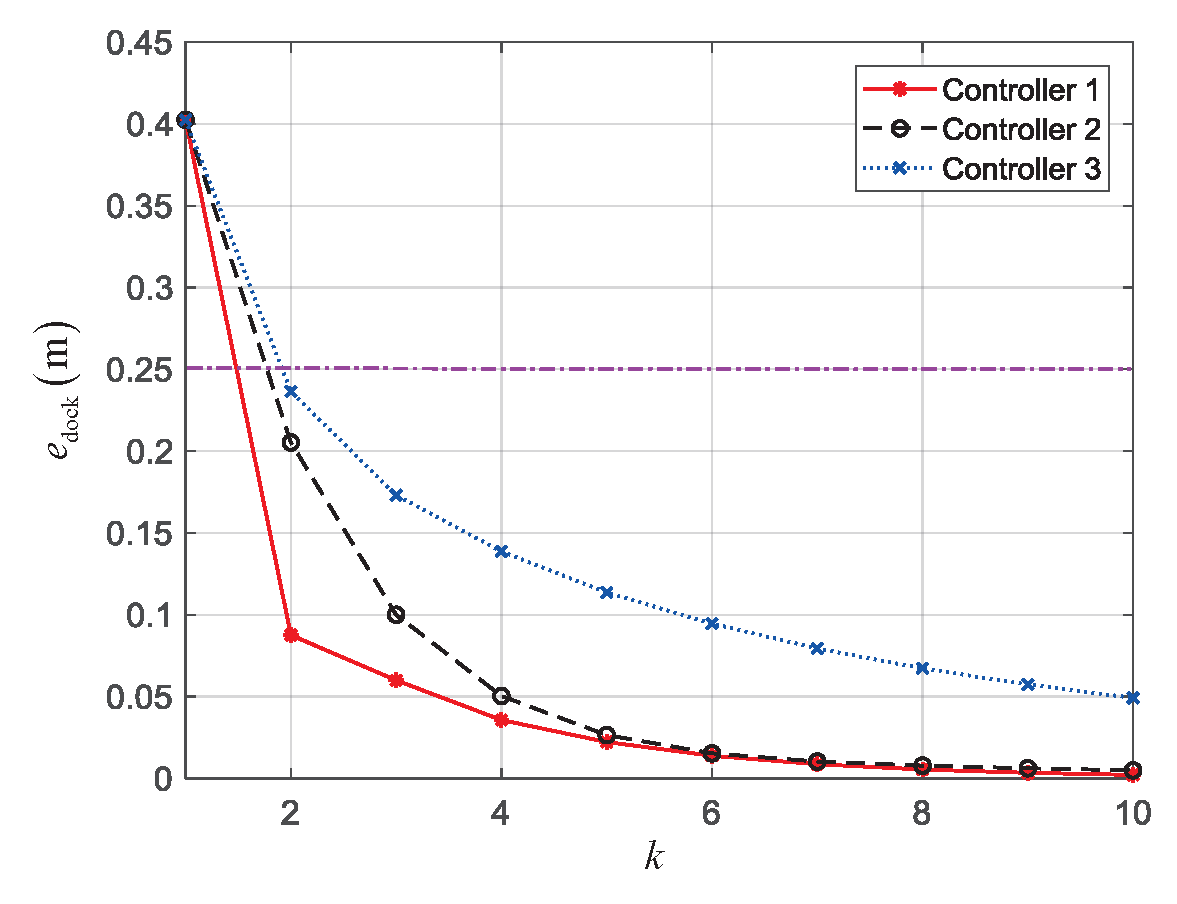
\includegraphics[width=0.6\textwidth]{Figures/Figs_Ch10/DockingError_Comp} 
		\par \end{centering}
	\caption{Comparison of the convergence of the terminal docking error between the proposed TILC controller (controller 1) and two traditional TILC controllers. (Since $r_{\text{d}%
		}=0.305$m as shown in Fig.~\ref{Fig_3Views}, a docking attempt is regarded
		as successful if the docking error is less than $0.25$m here.) }%
	\label{Fig_DockingError_Comp}%
\end{figure}

In the following, the simulation verification for the proposed hybrid TILC
controller will be focused on. The iterative process of the system outputs is
displayed in Fig.~\ref{Fig_DockingPosition}, which shows that the change of
initial position incurs a trajectory translation during the first half (before
the $20$s). While in the second half, not just a trajectory translation effect
is incurred because of the system nonlinearity and the change of control
inputs. Actually, the docking terminates at $t_{\text{end}}=30$s, and it is
for a better display to give the later outputs in the $30\sim50$s. It also can
be seen that the drogue deviates from the equilibrium position under the bow
wave effect when the receiver approaches the drogue. It is demonstrated in
Fig.~\ref{Fig_DockingPosition}(d) that the docking relative velocity stays
around -1.25 m/s at the docking moment. Because a good basis function is
selected, the velocity overshoot is small. The final successful
three-dimension docking trajectory is illustrated in Fig.~\ref{Fig_Docking3D}.
The probe successfully docks into the drogue in the end, and the solid red
line shows the motion of the moving drogue. \begin{figure}[pth]
	\begin{centering}
		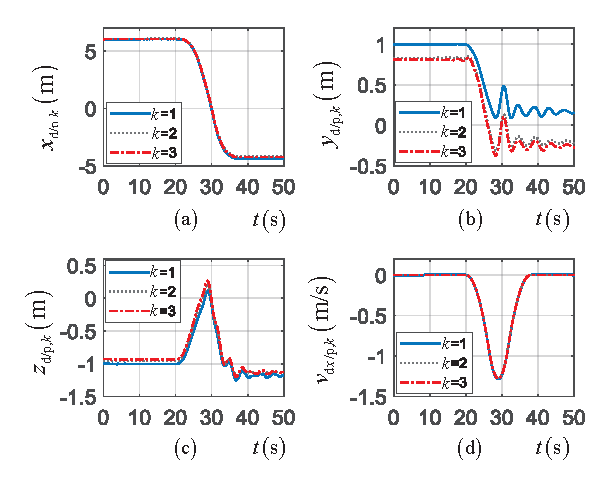
\includegraphics[width=0.6\textwidth]{Figures/Figs_Ch10/Out_C3} 
		\par \end{centering}
	\caption{The iteration of the relative position and relative velocity between the drogue and the probe during the docking process.}%
	\label{Fig_DockingPosition}%
\end{figure}\begin{figure}[pth]
	\begin{centering}
		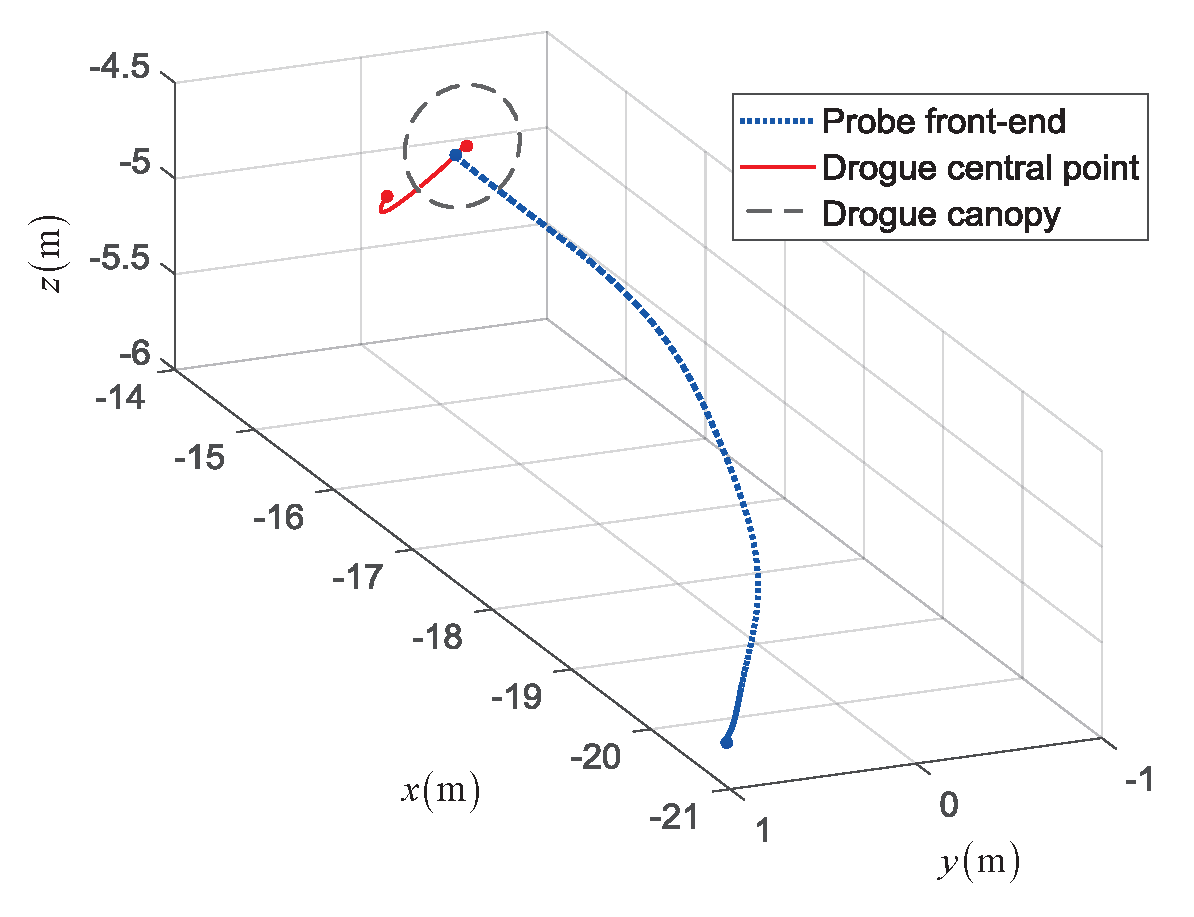
\includegraphics[width=0.6\textwidth]{Figures/Figs_Ch10/3DPath_C3} 
		\par \end{centering}
	\caption{A successful three-dimension docking trajectory of the probe and the drogue.}%
	\label{Fig_Docking3D}%
\end{figure}

\subsection{Simulation with uncertainties and disturbances}

In this part, in order to evaluate the robustness of the proposed hybrid TILC
controller, the following system uncertainties and disturbances are considered:

(i) Add uncertainties to actuators by multiplying actuator inputs by a factor
of 0.6, 0.8, 1.2, 1.4, respectively.

(ii) Change the actual bow wave effect to 1.2 times of the modeled bow
wave effect.

(iii) Add a side wind disturbance to the atmospheric environment.

(iv) Add the Dryden wind-turbulence model to the PDR system.

Noteworthy, the uncertainties (i), (ii) and disturbance (iii) are repetitive,
while the disturbance (iv) is stochastic and non-repetitive. The aforementioned four changes just apply to the plant, while controller design is still based on the model built
previously. Based on the uncertainties and disturbances (i), (ii), (iii) and
(iv), three scenarios are considered.

Scenario 1: Only the uncertainty (i) is considered.

Scenario 2: The actuator uncertainty factor is fixed to 0.6, and the uncertainties and
disturbances (ii), (iii) are also considered.

Scenario 3: The actuator uncertainty factor is fixed to 0.6, and the uncertainties and disturbances (ii), (iii), (iv) are all considered.

Under these scenarios, the convergence of the terminal docking error of the
proposed TILC controller is depicted in Figs.~\ref{Fig_C3_S1}-\ref{Fig_C3_S2}.
Fig.~\ref{Fig_C3_S1} shows that the convergence speed of the proposed TILC
controller decreases when there exist actuator uncertainties. The bigger the
actuator uncertainty is, the more the convergence speed decreases.
Fig.~\ref{Fig_C3_S2} shows that the docking error of the proposed TILC
controller can still converge to zero when there exist the uncertainties and
disturbances (i), (ii), (iii), which are repetitive. When there also exists the
stochastic uncertainty (iv), the docking error cannot converge to zero,
but it is bounded. The proposed TILC controller can achieve successful docking
at the third attempt, which illustrates that the proposed controller can
guarantee the docking performance under these uncertainties and
disturbances.\begin{figure}[pth]
	\begin{centering}
		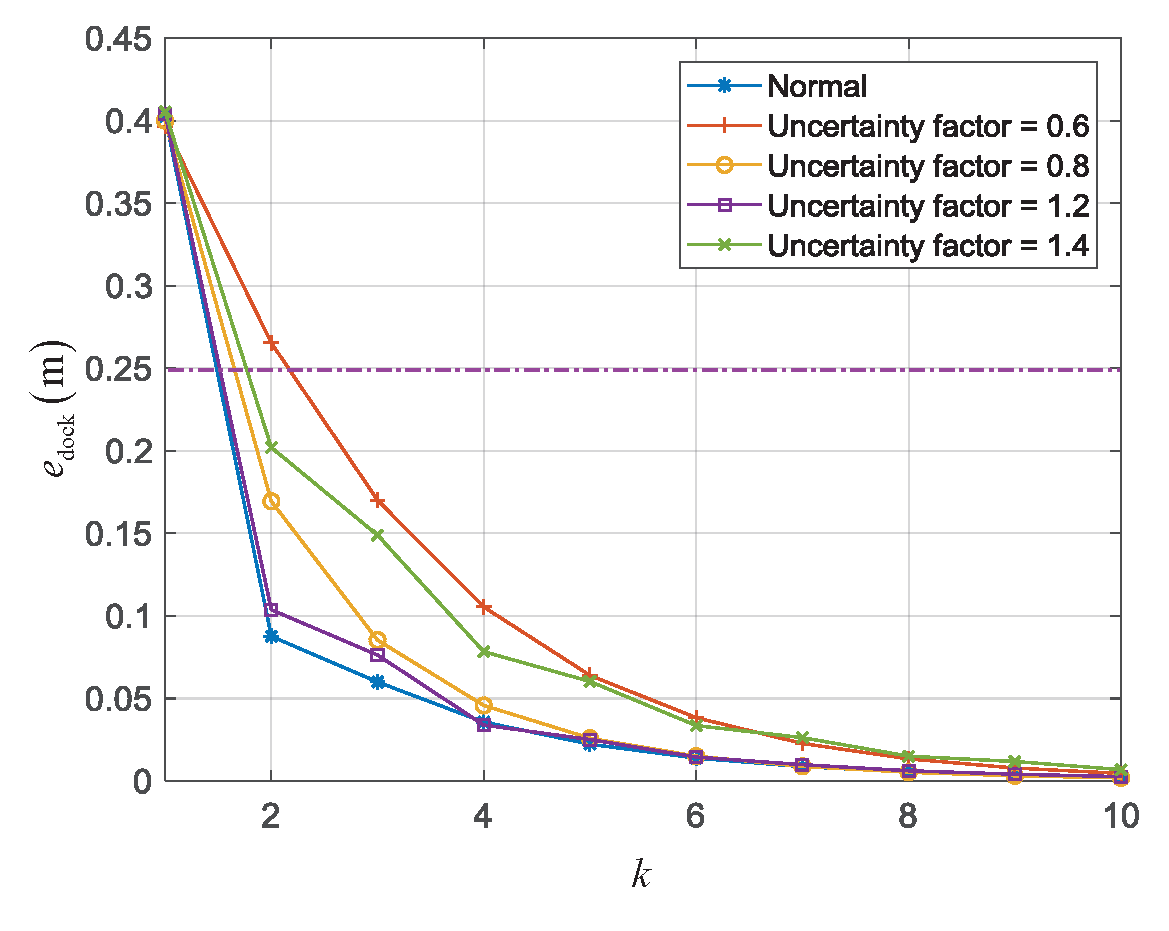
\includegraphics[width=0.6\textwidth]{Figures/Figs_Ch10/Scenario1} 
		\par \end{centering}\caption{Convergence of the terminal docking error when there exist actuator uncertainties (Scenario 1).}%
	\label{Fig_C3_S1}%
\end{figure}\begin{figure}[pth]
	\begin{centering}
		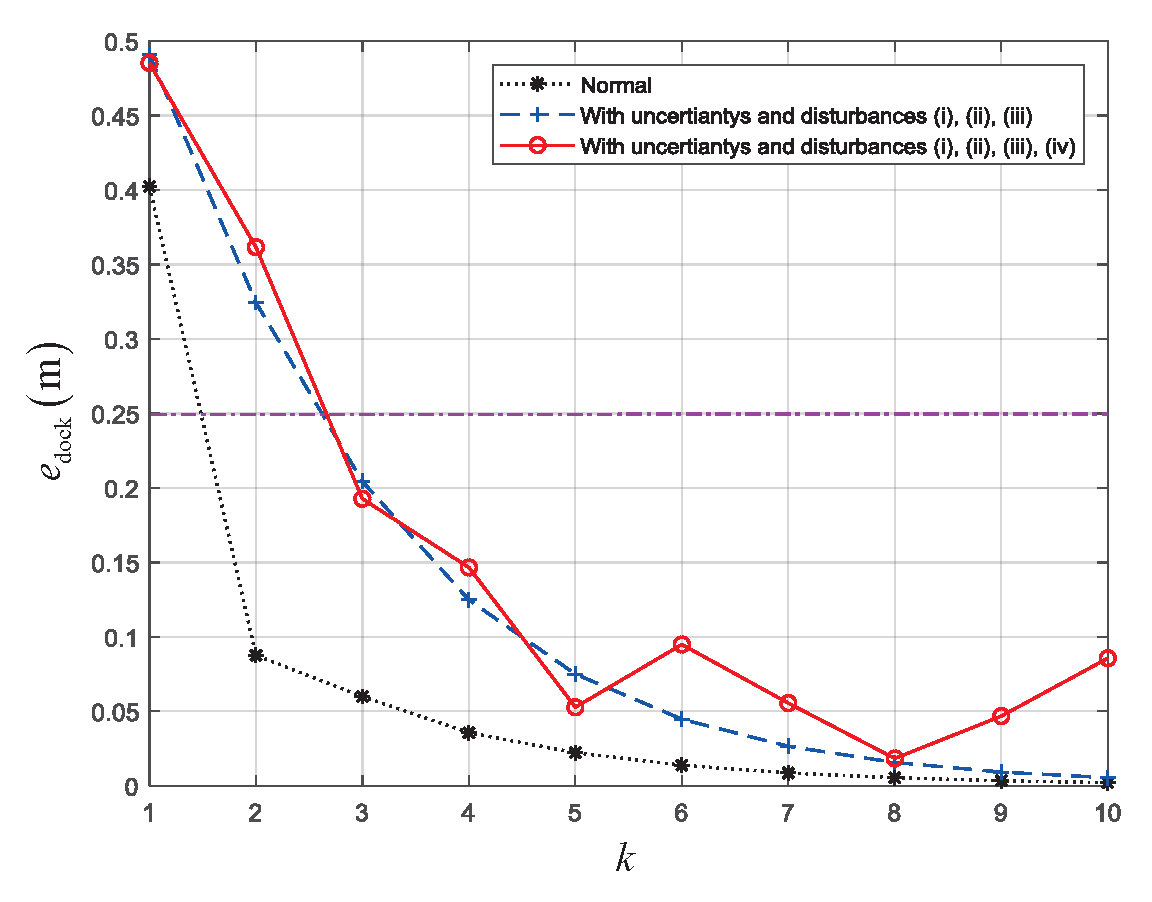
\includegraphics[width=0.6\textwidth]{Figures/Figs_Ch10/Scenario23} 
		\par \end{centering}\caption{Convergence of the terminal docking error when there exist uncertainties and uncertainties (Scenario 2 and Scenario 3).}%
	\label{Fig_C3_S2}%
\end{figure}

\subsection{Discussion}

The simulation exhibits favorable results. The proposed TILC controller does
not adopt real-time tracking method to track the moving drogue, so the problem
of the \textquotedblleft slow dynamics\textquotedblright \ to track the
\textquotedblleft fast dynamics\textquotedblright \ is solved. Because a good
basis function matrix is constructed in the preparation stage, the overshoot
at the docking moment is under control. Additionally, TILC is basically
model-free and robust, which can achieve successful docking without knowing
the drogue dynamics and the bow wave model. The proposed controller can also
provide successful docking in the presence of system uncertainties and
disturbances. These make the docking process safer and more reliable.

\section{Chapter Summary}

\label{Conclusions}

With the aim of achieving precise docking for the PDR system, a reliable
control scheme with a TILC docking control method is proposed to make the
receiver contact with the nonstationary drogue. The combination of control
inputs and initial state values is chosen as the learning object of TILC, and
the convergence condition is derived. The simulation results illustrate that
the docking precision is guaranteed after a few iteration cycles. Compared
with two traditional TILC controllers, the proposed hybrid TILC controller
gives the highest convergence speed.